\chapter{Future Work}


Active stress as function of eulerian fiber direction, not lagrangian \\
Global strain measures \\
full fledged heart sim \\
DTMRI \\
hemodynamics model \\
coupling with electrophysiology \\
contact with pericardium \\
FSI \\
coupling with cardiovascular simulation tools \\
coupling electrical, fluida \\
improvements to BCs, inside elastic medium \\
Lumens/SSA/active stress \\

%%%%%%%%%%%%%%%%%%%%%%
%%%%%%%%%%%%%%%%%%%%%%
\section{Towards Automating the Image-to-Analysis Pipeline}
\label{Towards Automating the Image-to-Analysis Pipeline}
%%%%%%%%%%%%%%%%%%%%%%
%%%%%%%%%%%%%%%%%%%%%%
\subsection{Multiple Materials and Inhomogeneous Materials}
\label{Multiple Materials and Inhomogeneous Materials}
%%%%%%%%%%%%%%%%%%%%%%
%%%%%%%%%%%%%%%%%%%%%%
\subsection{Uncertainty Quantification, Verification, and Validation}
\label{Uncertainty Quantification, Verification, and Validation}
Material properties, boundary conditions
%%%%%%%%%%%%%%%%%%%%%%
%%%%%%%%%%%%%%%%%%%%%%
\subsection{High Performance Computing}
\label{High Performance Computing}
%%%%%%%%%%%%%%%%%%%%%%
%%%%%%%%%%%%%%%%%%%%%%
\section{Clinical Implications}
\label{Clinical Implications}
(haptics, Simpleware stuff)\\
Center for Cardiovascular simulation (Texas)
Heartflow, Inc., Charles Taylor

ASME V\&V10 and V\&V40

dental applications - 1) for implant placement and crown design, 2) for 3D printing, aesthetic try-in 

tolerance-aware voronoi-partitioning \\
multiple material interfaces (see paper) \\

Abaqus: ability to deal with initial over-closures? A strain-free adjustment perhaps? Like if you were to mesh the femur and the femoral cartilage separately, say, and there is a tiny bit of overlap between them..are you able to fix this without going back to the meshing software?  

\begin{figure}[tbh]
\centering
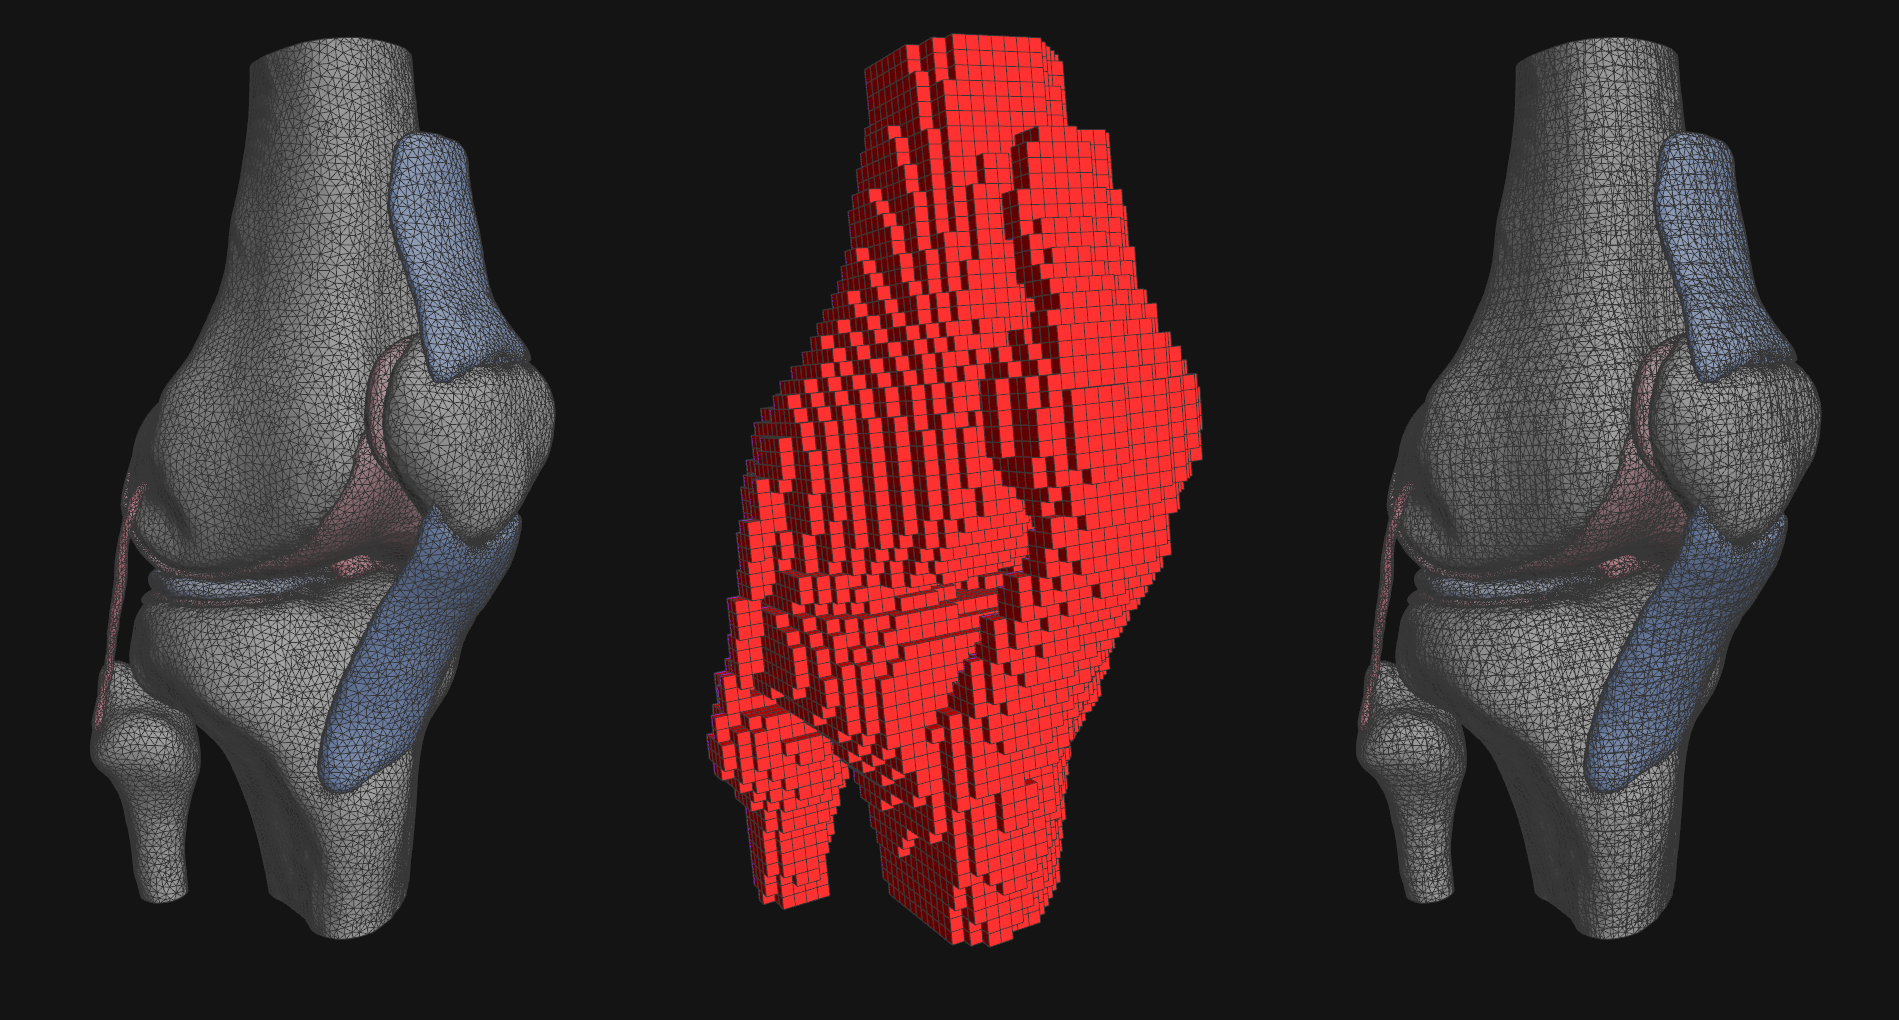
\includegraphics{media/sequence.png}
% where an .eps filename suffix will be assumed under latex,
% and a .pdf suffix will be assumed for pdflatex
\caption[sequence]{Polyhedral meshing sequence performed on knee mesh.}
\label{fig.sequence}
\end{figure}

\begin{sidewaysfigure}[tbh]
\centering
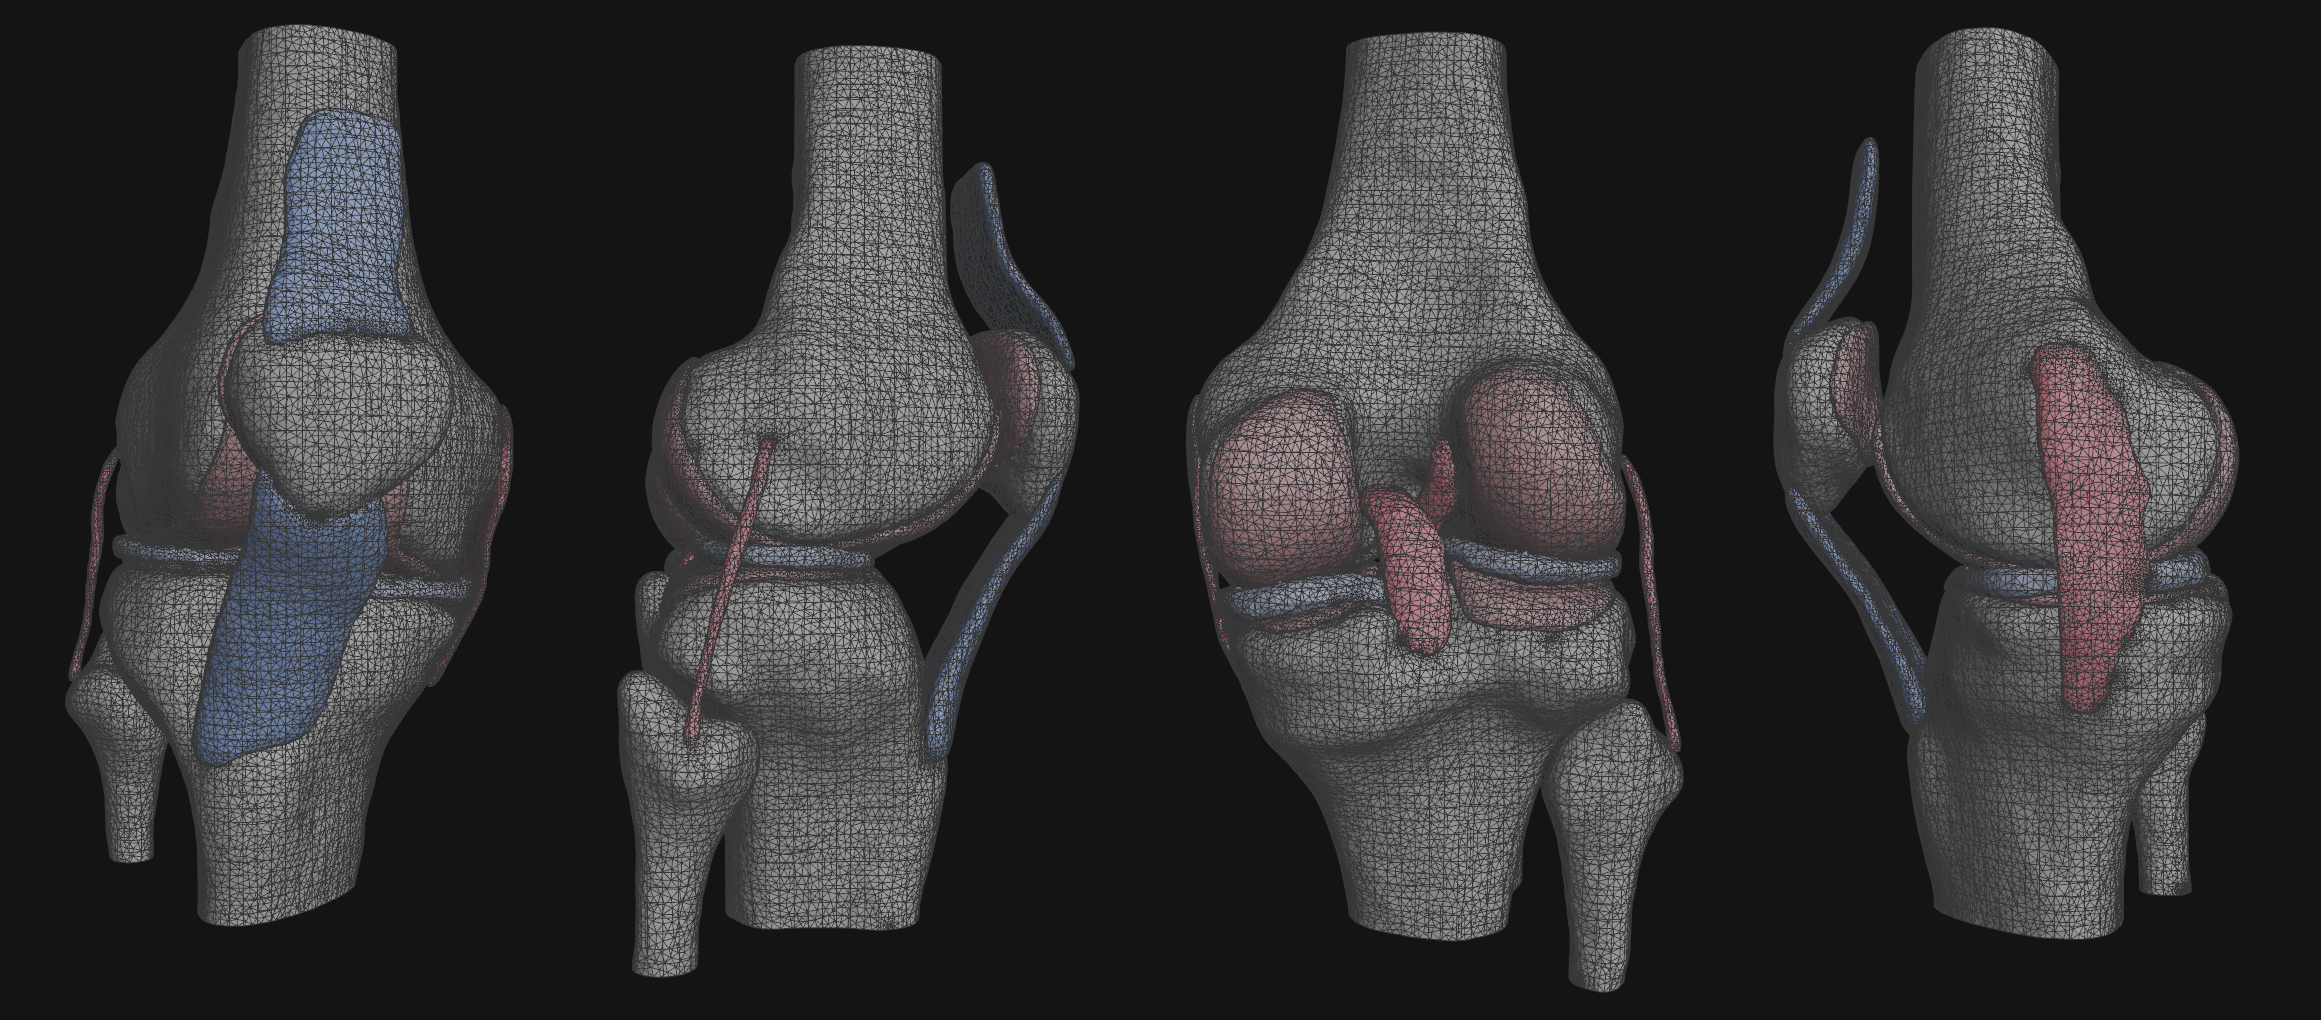
\includegraphics[scale=0.82]{media/fullmesh.png}
% where an .eps filename suffix will be assumed under latex,
% and a .pdf suffix will be assumed for pdflatex
\caption[polyhedral knee]{Resulting polyhedral mesh of knee.}
\label{fig.sample_1}
\end{sidewaysfigure}

Future Work

Comparison of surface reconstruction results to other methods \\
image-based meshing \\
Simplware \\
Cleaver \\
surface reconstruction \\
Poisson surf recon \\
vorocrust \\
tight cocone \\
compare volumes of segs to meshes \\
blender computes volume in 3D printing tab \\

\begin{table}[tbh]
% increase table row spacing, adjust to taste
\renewcommand{\arraystretch}{1.3}
% if using array.sty, it might be a good idea to tweak the value of
% \extrarowheight as needed to properly center the text within the cells
\centering
% Some packages, such as MDW tools, offer better commands for making tables
% than the plain LaTeX2e tabular which is used here.
\begin{tabular}{|c||c|}
\hline
One & Two\\
\hline
Three & Four\\
\hline
\end{tabular}
\caption[Example table]{An example of a table. Notice the caption is centered except when it runs longer than a single line on the page.}
\label{tab.example_1}
\end{table}